% template downloaded from https://kit-cd.sts.kit.edu/latex.php
% version: October 25, 2023
\documentclass[USenglish]{article} % package "babel" used for language handling

\usepackage{KITposter}
% package options:
% - "horizontal" (orientation)
% - "work" (add auxiliary lines for alignment)
% - "helvet", "heros" (use as main font)
% - "cursor" (use as typewriter font)

%\usepackage{amsmath} % mathematical symbols and equations; apparently pre-loaded
%\usepackage{amssymb} % mathematical symbols; apparently pre-loaded
%\usepackage{graphicx} % plots; apparently pre-loaded
\usepackage{tcolorbox} % colored boxes
%\usepackage{hyperref} % links and URLs; apparently pre-loaded

\graphicspath{{logos/}} % if not specified, logo is only searched in main folder

\title{\Huge\textcolor{KITgreen}{Subgroup Discovery with Small and Alternative Feature Sets}} % default title font size is \huge, which leads to last word being alone in second line; either use larger font size (\Huge) or smaller one (\LARGE)
\subtitle{SIGMOD 2025 | Berlin}
\author{\textcolor{KITgray}{Jakob Bach (\href{mailto:jakob.bach@kit.edu}{jakob.bach@kit.edu})}}
\institute{} % will be shown in top-right corner; warning if not provided
%\instadd{} % more institute information

\footline{} % content at end of poster; warning if not provided

\hypersetup{citecolor=KITblue, urlcolor=KITblue}

\newtcolorbox{standardbox}[1]{
	colback=white,
	colframe=KITgreen,
	boxsep=15pt, % padding added on all sides
	left=0pt, % padding added on specific side
	right=0pt,
	top=0pt,
	bottom=0pt,
	title={#1},
	fonttitle=\bfseries
}

\setlength{\leftmargini}{30pt} % increase space between bullet points and text
\setlength{\leftmarginii}{30pt}

\begin{document}

\maketitle

\begin{minipage}[t]{0.49\textwidth} % 1st column
	\vspace{0pt} % specifying vspace in both columns necessary to have them start at same y-position
	\begin{standardbox}{Scenario}
		\begin{itemize}
			\item \textbf{Problem:} Find interesting, simple-to-describe region(s) in dataset
		\end{itemize}
		%
		\centering
		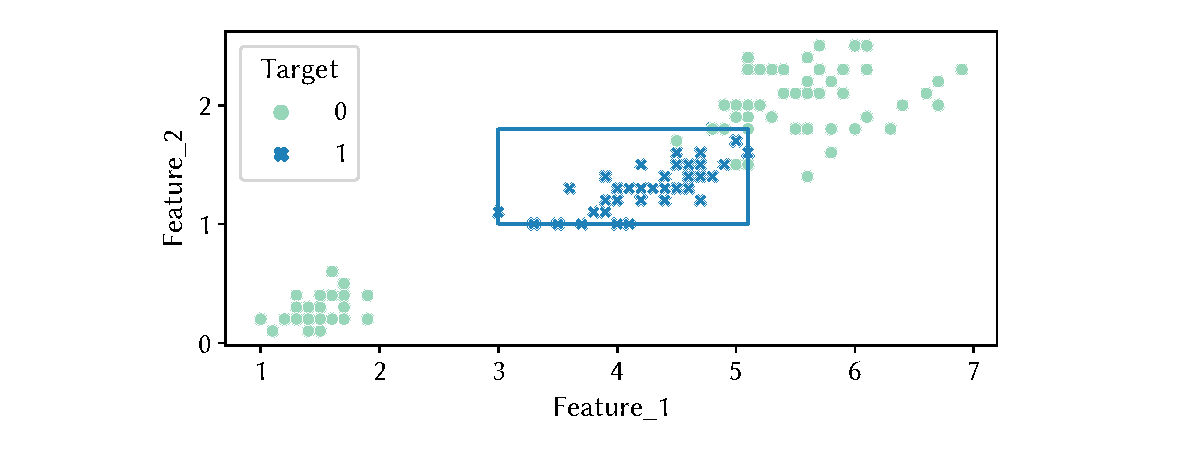
\includegraphics[width=0.95\textwidth, trim=70 10 90 10, clip]{plots/csd-exemplary-subgroup.pdf}
		%
		\begin{itemize}
			\item \textbf{Our scope:} Binary classification with real-valued features
			\begin{itemize}
				\item Tabular dataset $X \in \mathbb{R}^{m \times n}$ (data objects $\times$ features)
				\item Prediction target $y \in \{0, 1\}^m$ (`interesting'/`positive' = 1)
				\item Subgroup description: Hyperrectangle
				\item Subgroup quality: Weighted Relative Accuracy (WRAcc)
			\end{itemize}
			%
			\vspace{\baselineskip}
			%
			\item \textbf{Our focus}: Constraints for interpretable subgroup descriptions
		\end{itemize}
	\end{standardbox}
	%
	\vspace{10pt}
	%
	\begin{standardbox}{Contributions}
		\begin{itemize}
			\item Formalize subgroup discovery as an SMT optimization problem
			\item Formalize two constraint types (feature cardinality and alternatives)
			\item Analyze computational complexity and show $\mathcal{NP}$-hardness
			\item Comprehensive experiments
		\end{itemize}
	\end{standardbox}
	%
	\vspace{10pt}
	%
	\begin{standardbox}{Formalization -- Basic Problem}
		\begin{align*}
			\max &\quad & Q_{\text{WRAcc}} &= \frac{m_b}{m} \cdot \left( \frac{m_b^+}{m_b} - \frac{m^+}{m} \right) = \frac{m_b^+}{m} - \frac{m_b \cdot m^+}{m^2} \\
			\text{s.t.:} &\quad & m_b &:= \sum_{i=1}^{m} b_i \quad\text{and}\quad m_b^+ := \sum_{\substack{i \in \{1, \dots, m\} \\ y_i = 1 }} b_i \\
			&\quad \forall i \in \{1, \dots, m\} & b_i &\leftrightarrow \bigwedge_{j \in \{1, \dots, n\}} \left( \left( X_{ij} \geq \mathit{lb}_j \right) \land \left( X_{ij} \leq \mathit{ub}_j \right) \right) \\
			&\quad \forall j \in \{1, \dots, n\} & \mathit{lb}_j &\leq \mathit{ub}_j \\
			&\quad & b &\in \{0, 1\}^m \\
			&\quad & \mathit{lb}, \mathit{ub} &\in \{\mathbb{R} \cup \{-\infty, +\infty\}\}^n
		\end{align*}
	\end{standardbox}
	%
	\vspace{10pt}
	%
	% QR codes generated with https://www.qrcode-monkey.com/
	\setlength{\tabcolsep}{80pt} % increase space between columns
	\centering
	\begin{tabular}{ccc} % using floats (via "subcaption") does not work
		
\includegraphics[width=0.15\textwidth]{qr_codes/qr-code-paper.pdf} &
		
\includegraphics[width=0.15\textwidth]{qr_codes/qr-code-github.pdf} &
		
\includegraphics[width=0.15\textwidth]{qr_codes/qr-code-data.pdf} \\
		\href{https://doi.org/10.1145/3725358}{Paper} &
		\href{https://github.com/Jakob-Bach/Constrained-Subgroup-Discovery}{Code} &
		\href{https://doi.org/10.35097/nftgaf7w73hy2491}{Data} \\
	\end{tabular}
\end{minipage}
%
\hfill
%
\begin{minipage}[t]{0.49\textwidth} % 2nd column
	\vspace{0pt}
	\begin{standardbox}{Constraints to Foster Interpretability}
		\begin{itemize}
			\item \textbf{Feature-cardinality constraints:}
			\begin{itemize}
				\item Limit number of features used in subgroup description to $k \in \mathbb{N}$
				\item Feature used if its bounds exclude $\geq 1$ data object from subgroup
			\end{itemize}
			%
			\vspace{\baselineskip}
			%
			\item \textbf{Alternative subgroup descriptions:}
			\begin{itemize}
				\item New optimization problem: Cover similar set of data objects as a given subgroup but use different feature set in description
				\item Parameters: Number of alternatives~$a$, dissimilarity threshold~$\tau$
			\end{itemize}
		\end{itemize}
	\end{standardbox}
	%
	\vspace{10pt}
	%
	\begin{standardbox}{Experimental Design}
		\begin{itemize}
			\item 27 datasets from \emph{PMLB} (with $m \in [106, 9822]$ and $n \in [20, 168]$)
			\item 8 subgroup-discovery methods: SMT-solver-based and 7 competitors
			\item Vary parameter values for constraints ($k$, $a$, $\tau$) and solver's timeout
		\end{itemize}
	\end{standardbox}
	%
	\vspace{10pt}
	%
	\begin{standardbox}{Experimental Results: Feature-Cardinality Constraints}
		\centering
		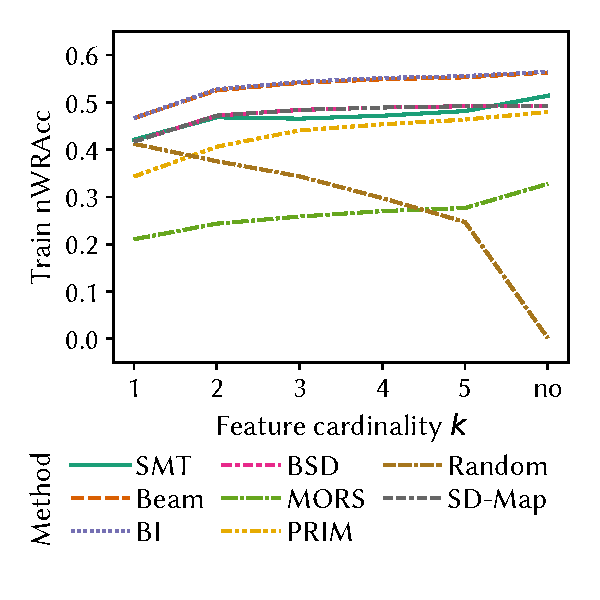
\includegraphics[width=0.48\textwidth, trim=10 25 10 10, clip]{plots/csd-cardinality-train-nwracc-all-datasets.pdf}
		\hfill
		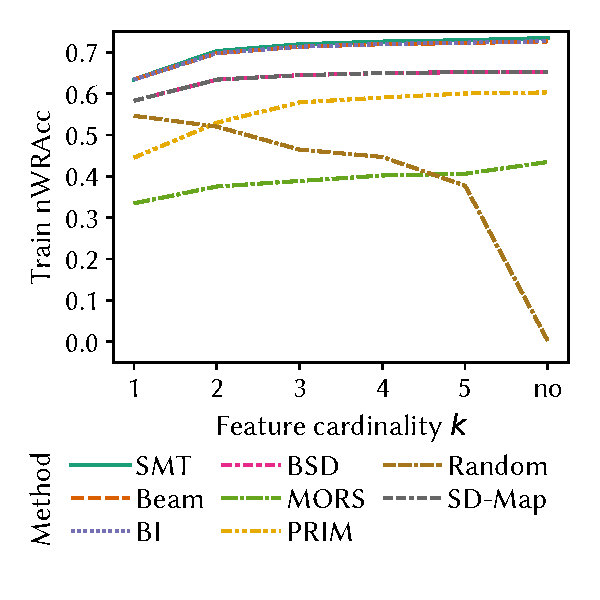
\includegraphics[width=0.48\textwidth, trim=10 25 10 10, clip]{plots/csd-cardinality-train-nwracc-no-timeout-datasets.pdf}
		%
		\begin{itemize}
			\item Left: all datasets; right: only datasets without solver timeouts
			\item Heuristics \emph{Beam} and \emph{BI} yield high subgroup quality (WRAcc) fast
			\item Using few features suffices to reach high subgroup quality
		\end{itemize}
	\end{standardbox}
	%
	\vspace{10pt}
	%
	\begin{standardbox}{Experimental Results: Alternative Subgroup Descriptions}
		\centering
		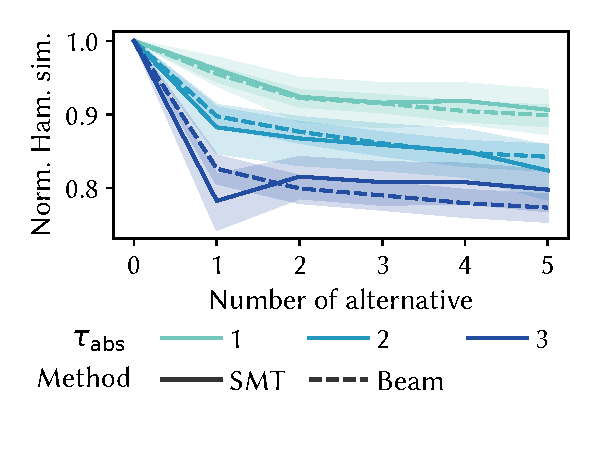
\includegraphics[width=0.48\textwidth, trim=10 25 10 10, clip]{plots/csd-alternatives-hamming.pdf}
		\hfill
		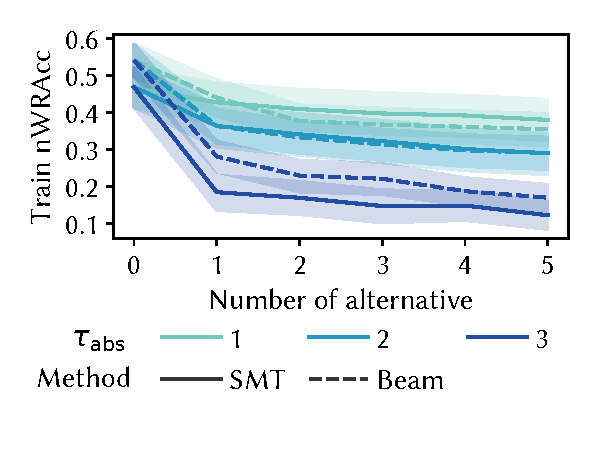
\includegraphics[width=0.48\textwidth, trim=10 25 10 10, clip]{plots/csd-alternatives-train-nwracc.pdf}
		%
		\begin{itemize}
			\item Left: similarity to original subgroup; right: subgroup quality
			\item Similarity and quality of alternatives decreases over~$a$ and~$\tau$
			\item Strongest decrease from original subgroup to first alternative
		\end{itemize}
	\end{standardbox}
\end{minipage}

\end{document}
